\documentclass[a4paper, 11pt]{article}
\usepackage{comment} 
\usepackage{fullpage} 
\usepackage[spanish]{babel} 
\selectlanguage{spanish}
\usepackage[utf8]{inputenc}
\usepackage{float} 
\usepackage{graphicx}
\usepackage{ marvosym }
\usepackage{amsthm}
\usepackage{amsmath}
\usepackage[sort&compress, numbers]{natbib}
\usepackage{amssymb}
\usepackage{hyperref}
%\hypersetup{colorlinks=True, citecolor=blue}
\hypersetup{colorlinks=true, citecolor=green, urlcolor=blue}

\begin{document}
\begin{center}
\LARGE \bf Pr\'actica 10\\ Algoritmo genético
\end{center}

\vspace{1cm} 
\noindent\textbf {Edson Edgardo Samaniego Pantoja} \hfill \textbf{Materia:} Simulación computacional 
\hfill \\
\textbf{Fecha} \today  
\vspace{1cm} 

\section{Introducción}
El método o problema de la mochila conocido como (\texttt{knapsack}), es un problema de optimización el que consiste en seleccionar un subconjunto de objetos de tal forma que la capacidad no se exceda de la mochila sumando los pesos de los objetos incluidos pero que el valor total de los objetos sea lo máximo posible. 
En cuanto al algoritmo genético es una técnica de programación que imita a la evolución biológica como estrategia para resolver problemas. Dado un problema específico a resolver, la entrada del algoritmo genético es un conjunto de soluciones potenciales a ese problema, codificadas de alguna manera, y una métrica llamada función de aptitud que permite evaluar cuantitativamente a cada candidata. Estas candidatas pueden ser soluciones que ya se sabe que funcionan, con el objetivo de que el AG las mejore, pero se suelen generar aleatoriamente.
Un algoritmo genético consiste en una función matemática o una rutina de software que toma como entradas a los ejemplares y retorna como salidas cuales de ellos deben generar descendencia para la nueva generación.
\section{Objetivo}
El objetivo en la práctica es cambiar la selección de los padres para reproducción a que utilice seleccion de ruleta, cada solución se selecciona como padre con una probabilidad que es linealmente proporcional a su valor de función objetivo y a su factibilidad combinando los dos a alguna función que parezca conveniente e inversamente proporcional a alguna combinación de factibilidad y objectivo para la mutación.

Lo siguiente es generar tres distintas reglas:
\begin{itemize}
    \item el peso y el valor de cada objeto se generan independientemente con una distribución normal,
    \item el valor de cada objeto se generan independientemente con una distribución exponencial y su peso es inversamente correlacionado con el valor, con un ruido normalmente distribuido de baja magnitud,
    \item el peso de cada objeto se generan independientemente con una distribución normal y su valor es (positivamente) correlacionado con el cuadrado del peso, con un ruido normalmente distribuido de baja magnitud.
\end{itemize}

Como final es determina para cada uno de los tres casos a partir de qué tamaño de instancia el algoritmo genético es competitivo con el algoritmo exacto en términos de valor total obtenido por segundo de ejecución.

\section{Simulación}
El código base es dado en el repositorio de Schaeffer \cite{elisa} que de igual manera se puede consultar en la pagina web \cite{dra} donde se explica cada código paso a paso.
El primer cambio realizado al programa original es la creación de un ciclo \texttt{for} que varía las reglas dando un total de tres iteraciones.

Dentro del ciclo son tres ciclos \texttt{if} para cada regla cada uno genera para cada caso los pesos y valores, en el primero independientes, segundo los valores son independientes con una distribución exponencial y el tercero serán los valores correlacionados con el cuadrado del peso.

\begin{verbatim}
for regla in (1, 2, 3):
    pesosexp=[]
    diferentes=[]
    vdif=[]
    vd=[]
    ANTES= time()
    
    if regla == 1:
        n=50
        pesos = generador_pesos(n, 15, 80)
        for B in range(0,len(pesos)):
            diferentes.append(randint(0,300))
        valores = generador_valores(diferentes, 10, 500)
  
    if regla == 2:
        n=300
        for C in range(0,n):
            vdif.append(randint(0,20))
        for D in range(0, n):
            vd.append(math.exp(vdif[D]))
        pesos = generador_pesos(n, 15, 80)
        valores = generador_valores(vd, 10, 500)

    if regla == 3:
        n=150
        pesos = generador_pesos(n, 15, 80)# genera 50 aleatorio en rango de 15 a 80
        for A in range(0,len(pesos)):
            pesosexp.append(pesos[A]**2)
        valores = generador_valores(pesosexp, 10, 500)#50 valores entre 10 a 500

\end{verbatim}

Después el siguiente cambio es un ciclo que tendrá dos repeticiones ya que en la primera se hará el proceso de generar mutaciones y reproducción de manera normal y para el segundo ciclo se utilizara la función de \texttt{ruleta}.

\begin{verbatim}
    for ciclo in range(0,2): 
        init = 200
        p = poblacion_inicial(n, init)
        tam = p.shape[0]
        assert tam == init
        pm = 0.05
        rep = 50
        tmax = 50
        mejor = None
        mejoresruleta=[]
        for t in range(tmax):
            d = []
            for i in range(tam):
                d.append({'idx': i, 'obj': objetivo(p[i], valores),
                          'fact': factible(p[i], pesos, capacidad)})

            d = pd.DataFrame(d).sort_values(by = ['fact', 'obj'], ascending = False)
            listaR=pd.DataFrame(d).sort_values(by=['idx'], ascending=0)
    
            for i in range(rep):  
                if ciclo == 0:
                    padres = sample(range(tam), 2)
                if ciclo == 1:
                    padres= ruleta(d,tam)
                hijos = reproduccion(p[padres[0]], p[padres[1]], n)
                p = np.vstack([p, hijos[0], hijos[1]])
\end{verbatim}

La función ruleta es creada de manera que se ingresa una lista que contiene el \texttt{dataframe} que ordena los valores objetivos tanto falsos como verdaderos de menor a mayor y la variable \texttt{n}. Dentro de la función primeramente se toma el largo de cada conjunto de objetivos (falso y verdadero) para que cada uno en un ciclo \texttt{for} acumule enumeradamente la cantidad de datos. De cada lista se extraen dos valores al azar con la función \texttt{sample}, en otra variable se utiliza \texttt{random choices} para seleccionar al azar uno de estos resultados del \texttt{sample} pero con la diferencia que tendrá una probabilidad según la cantidad de verdaderos y falsos. Los ciclos \texttt{if} son para cuando el \texttt{random choices} selecciona resultados del mismo tipo de listas o uno de cada uno, si es el primer caso tomará dos valores distintos ya que se realizo un \texttt{sample} previamente.
\begin{verbatim}
def ruleta(lista,n):
    import random
    F, NF = [],[]
    f=len(lista.loc[lista.fact == True,])
    nf=len(lista.loc[lista.fact == False,])
    for i in range(0,f):
        F.append(i)
    for j in range(f,(f+nf)):
        NF.append(j)

    listas=[(random.sample(F, k=2)),(random.sample(NF, k=2))]
    results= random.choices(listas, weights= [len(F), len(NF)], k = 2)
    if results[0]==results[1]:
        salida= results[0]
    if results[0]!=results[1]:
        dato1= results[0]
        dato2= results[1]
        salida= [dato1[0],dato2[0]]
    return(salida)
\end{verbatim}

El código completo puede ser encontrado en github \cite{Edson}.

\section{Resultados}

Los resultados son mostrados en la tabla \ref{tab1} la cual aplica para las tres reglas y por cada regla se ven los mejores resultados con y sin ruleta y cuanto tiempo tardo según su valor de \texttt{n} el cual fue dado de manera que la gráfica se acercara más al valor óptimo. 

    \begin{table}[H]
        \caption{Registro de posición, carga, masa y velocidad promedio por paso de cada partícula.}
        \bigskip
        \label{tab1}
        \centering
        \begin{tabular}{|r|r|r|r|r|r|}
        \hline
         Regla&n&Sin ruleta&Ruleta&Óptimo&Tiempo (s)\\
        \hline
        1 & 50 & 10432.13 & 10277.88 & 10473.00 & 3.55 \\
        \hline
        2 & 350 & 14054.90 & 13841.42 & 14448.10 & 13.15 \\
        \hline
        3 & 60 & 9324.69 & 9356.22 & 9527.11 & 3.84 \\
        \hline
        \end{tabular}
    \end{table}

Los siguientes gráficos figuras \ref{f1}, \ref{f2}, \ref{f3} se puede observan en franja horizontal verde el valor óptimo y dos lineas punteadas azul y roja para los resultados sin ruleta y con ruleta respectivamente.

\begin{figure}[H]
  \centering      
  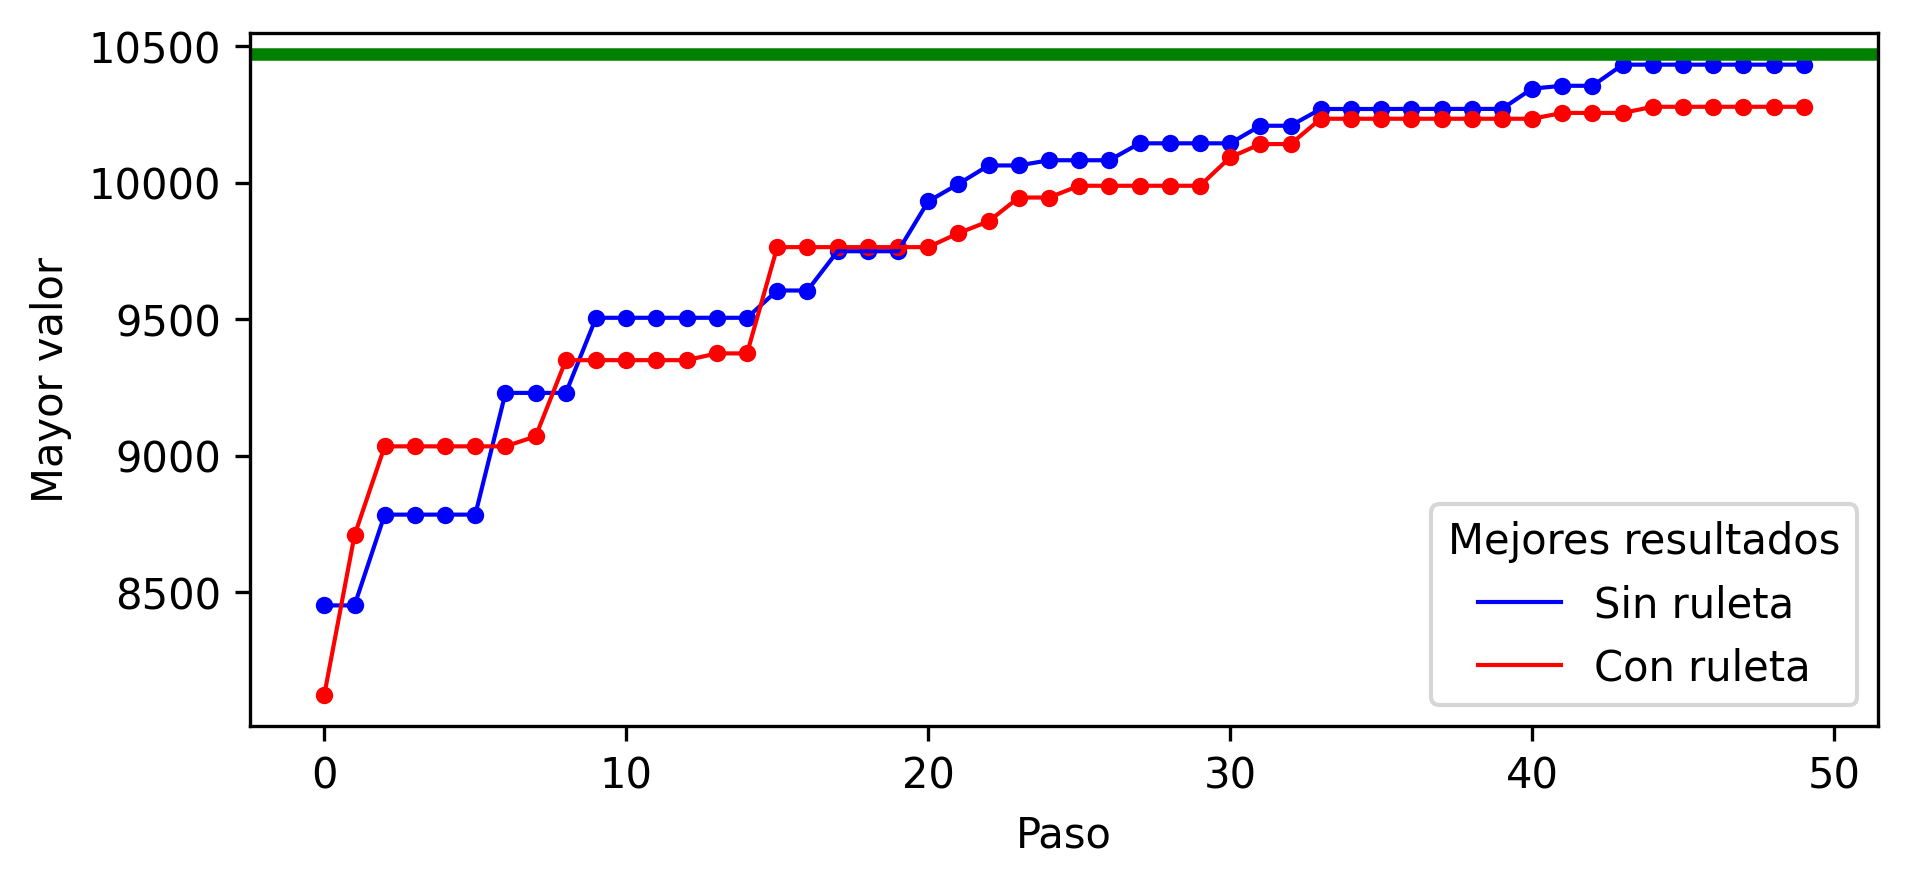
\includegraphics[scale=.9]{regla_1.png}
  \caption{Gráfica de los mejores valores para regla 1}
  \label{f1}
\end{figure}
\bigskip

\begin{figure}[H]
  \centering      
  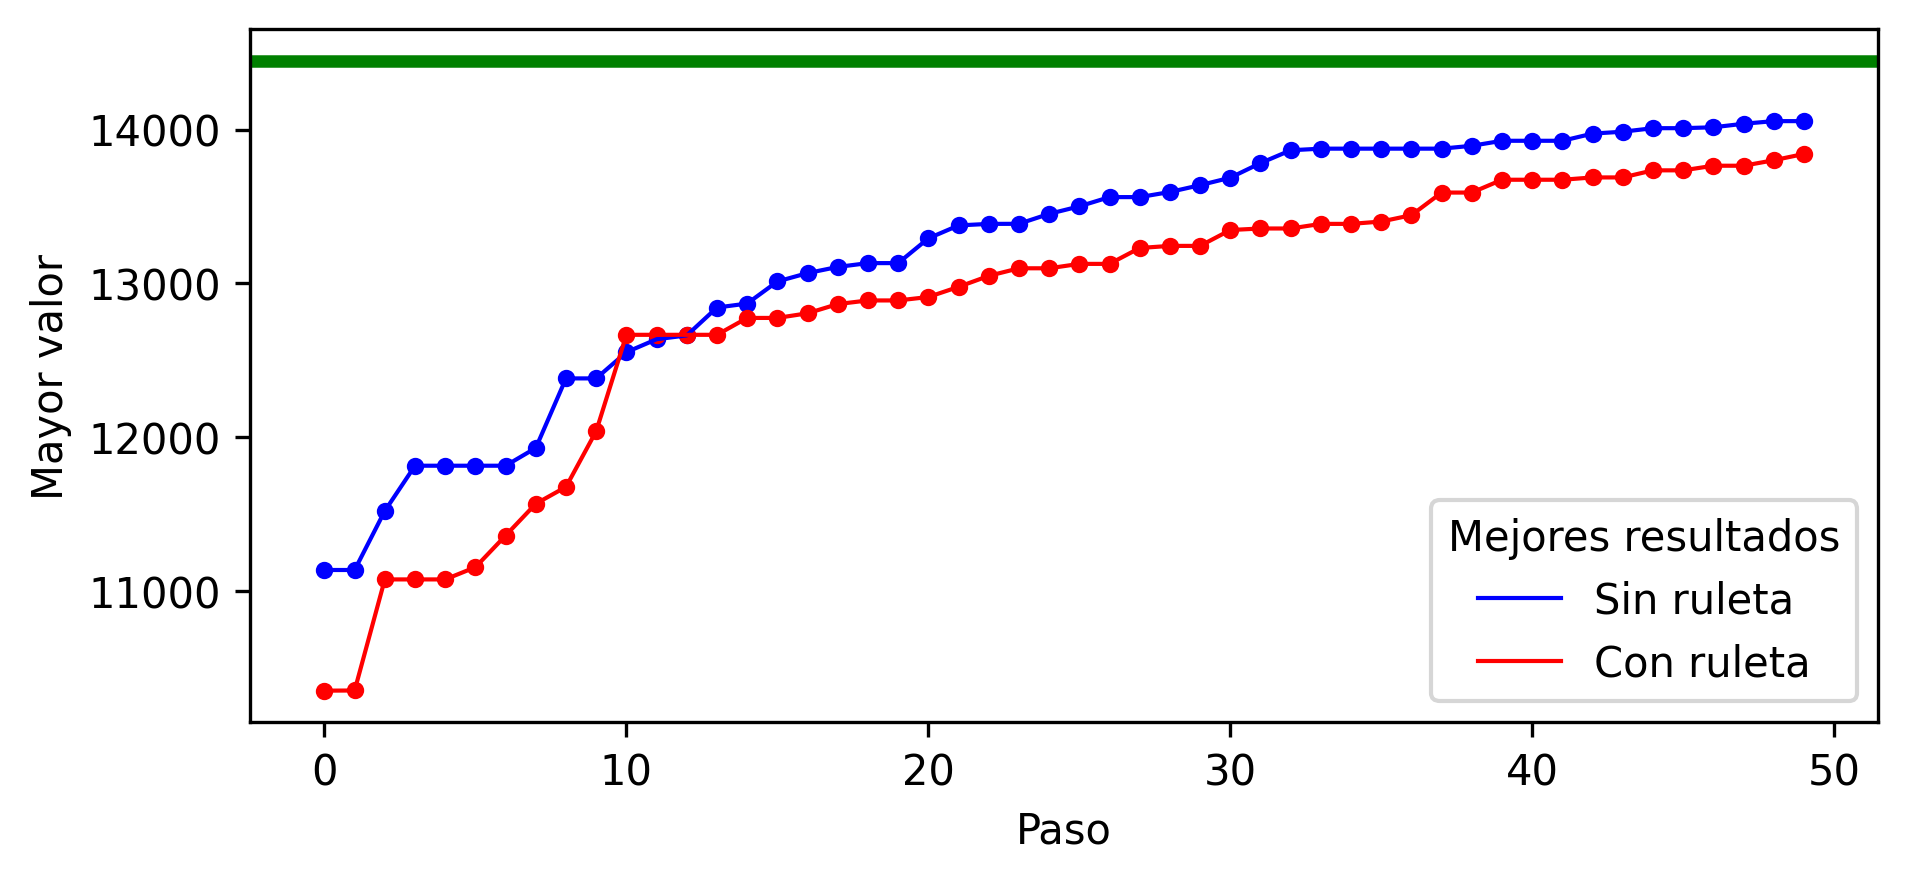
\includegraphics[scale=.9]{regla_2.png}
  \caption{Gráfica de los mejores valores para regla 2}
  \label{f2}
\end{figure}
\bigskip

\begin{figure}[H]
  \centering      
  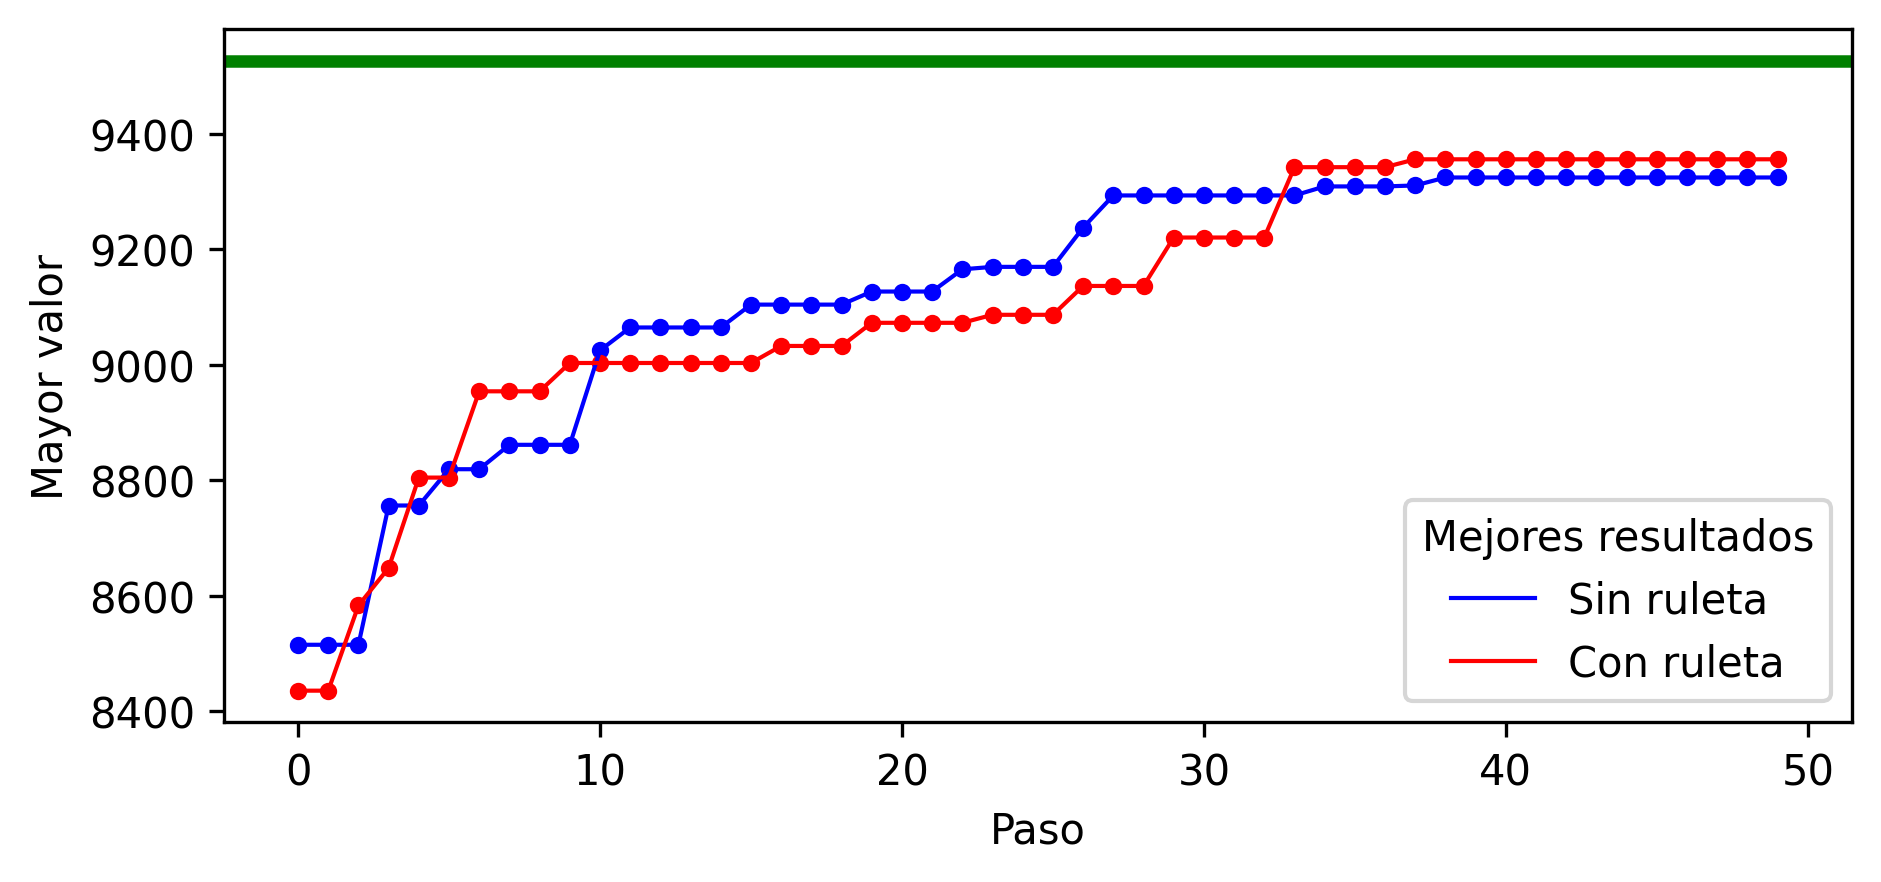
\includegraphics[scale=.9]{regla_3.png}
  \caption{Gráfica de los mejores valores para regla 3}
  \label{f3}
\end{figure}
\bigskip

\section{Conclusión}

Se puede concluir en base a las figuras, la regla con la que hubo mejores resultados es la uno dando valores muy cercanos al óptimo dando diferencias de 40.87 sin ruleta y con ruleta 195.17 que si bien no llega el algoritmo genético a un valor óptimo, se tiene una mejora utilizando el método de mochila.

Algo que se observa en común en dos gráficos para la regla uno y dos es que el utilizar la ruleta para seleccionar de manera al azar porcentualmente los resultados, no le beneficia del todo a lo cual no rebasa en mejoría que si se hace la reproducción sin ruleta.

La ultima regla la cual relaciona pesos y valores siendo estos últimos elevaciones al cuadrado, hace una cercanía en las dos lineas punteadas en la gráfica \ref{f3} por lo que apartir del paso treinta comienzan a comportarse linealmente y muy cercanas en sus valores.

\bibliography{refe}
\bibliographystyle{plainnat}

\end{document}

